\documentclass[12pt,a4paper,twoside,openright,pdftex]{book}
                              % Reproservice prints on G4, which is about 80% of A4.
                              % With this scale, 12pt font becomes 9.6pt.
                              % https://www.chalmers.se/insidan/SV/arbetsredskap/kommunikation/tryck-och-layout/mallar-for-trycksaker/avhandlingens-utformning

\synctex=1                    % instead of "pdflatex -synctex=1 main"

\usepackage{lipsum}           % generating fill-in text for this thesis template

\usepackage{ifthen}           % if-then-else (to choose PhD/Lic titles)

\usepackage[utf8]{inputenc}   % unicode letters in the input tex document

\usepackage[T1]{fontenc}      % unicode letters in the output pdf

\usepackage{amssymb, amsmath} % math symbols

\usepackage{lmodern}          % better font

\usepackage{microtype}        % micro typesetting (on errors use draft to disable)

\usepackage{booktabs}         % better table formatting

\usepackage[pdftex]{graphicx} % images

\usepackage{tikz}             % simply amazing graphics library for LaTeX
\usetikzlibrary{calc}

\usepackage[%                 %
  a4paper%
  ,twoside                    %
  ,inner=2.5cm                % inner margin
  ,outer=2.5cm                % outer margin
  ,bindingoffset=1cm       % additional binding offset on the inner side
  ,bottom=3cm
]{geometry}                   % Adjust the margins

\usepackage{fancyhdr}         % fine-tuning of headers
\pagestyle{fancy}

\usepackage{emptypage}        % no page numbers in headers/footers of blank pages between chapters

\usepackage{setspace}         % for \setstretch in captions

\usepackage[%
    margin=0.75cm,            % make captions narrower than the main text
    font={small,stretch=0.80}%%
  ]{caption}                  % captions

\usepackage{subcaption}       % subcaption -- subfigures (replaces subfig)

\usepackage{url}              % handles URLs correctly (e.g. DOI, software links)

\usepackage[%
  url=true,%                  % print URLs in references, except for the ones removed below
  backend=biber,%             % use biber instead of bibtex
  style=authoryear,%          % cite as: (Author 2008)
  maxbibnames=10,%            % max names in bibliography
  maxcitenames=2,%            % max names in citation
  mincitenames=1,%            % if there are more than maxcitenames, shrink to this
  backref=true,%              % prints page numbers (wrong with \frontmatter and hypertexnames=false)
  dashed=false                % do not replace repeated author with a dash in bibliography
]{biblatex}                   % Modern bibtex replacement (bibliography mgmt)

\usepackage[%
   pdftex%
  ,hidelinks%
  ,linktoc=all%               % part of a ToC entry to be made into a link (section/page/all)
  ,unicode%
  ,bookmarksopen=true%
  ,bookmarksopenlevel=0
  ,bookmarksnumbered=true
  %,hypertexnames=false,%     % Correct ToC hyperlinks even with chapter counter reset, but broken biblatex backref.
                              % Instead of using hypertexnames=false, use \renewcommand on \theHchapter, 
                              % see http://tex.stackexchange.com/a/6099
  %,draft                     % draft can be used to avoid some strange links errors
]{hyperref}                   % links in pdf document

\usepackage{bookmark}         % Create pdf bookmarks in one go

\usepackage{physics}
\usepackage{pdfpages}

% % % Biblatex

\addbibresource{library.bib}  % Bibliography file
\renewcommand{\cite}{\parencite}

% Remove URLs from common (easy-to-find) entries.
\AtEveryBibitem{%
  \ifboolexpr%
    {%
      test { \ifentrytype{book} }
      or
      test { \ifentrytype{inbook} }
      or
      test { \ifentrytype{inproceedings} }
      or
      test { \ifentrytype{incollection} }
      or
      test { \ifentrytype{article} }
    }
    {\clearfield{url}}
    {}%
}
% End Biblatex


% % % New environments

% \newenvironment{env-name}[optional-number-of-args]{insert-before}{insert-after}

% \newenvironment{env-name}[optional-number-of-args][default-args]{insert-before}{insert-after}

\newenvironment{abstract}{
  \begin{center}
    {\bfseries Abstract\par}  % \bfseries - some bold font, \par - end of paragraph (as empty line)
  \end{center}
  \quotation                  % extra indent from left and right
  \noindent
}
{\par\endquotation}

\newenvironment{keywords}%
{{\bfseries Keywords:}}%
{\par}%
% % % End new environments


% Begin page content adjustments for putting more text on pages.
\renewcommand{\topfraction}{.85}       % max fraction of floats at top
\renewcommand{\bottomfraction}{.7}     % max fraction of floats at bottom
\renewcommand{\textfraction}{.15}      % minimal text wrt. figs
\renewcommand{\floatpagefraction}{.66} % fraction for page of floats. floatpagefraction MUST be less than topfraction 
\renewcommand{\dbltopfraction}{.66}    % fit big float above 2-col. text
\renewcommand{\dblfloatpagefraction}{.66}
\setcounter{topnumber}{9}
\setcounter{bottomnumber}{9}
\setcounter{totalnumber}{20}
\setcounter{dbltopnumber}{9}
\widowpenalty=300                             % widow (at the beginning of page)
\clubpenalty=300                              % orphans (at the end of page)
\setlength{\parskip}{0ex plus 0.5ex}  % space between paragraphs
% End page content adjustments

% % %
% Begin remove page numbers from the "Part I" pages
\fancypagestyle{veryempty}{% no headers, no page numbers
  \fancyhf{} % remove everything
  \fancyfoot{}
  \renewcommand{\headrulewidth}{0pt} % remove lines as well
  \renewcommand{\footrulewidth}{0pt}
}
\makeatletter
\renewcommand\part{%
  \if@openright
    \cleardoublepage
  \else
    \clearpage
  \fi
  \thispagestyle{veryempty}%
  \if@twocolumn
    \onecolumn
    \@tempswatrue
  \else
    \@tempswafalse
  \fi
  \null\vfil
  \secdef\@part\@spart}
\makeatother
% End remove page numbers from the "Part I" pages


% % % % %

% Common things used both in the thesis and in the defence announcement

\newcommand\thesistype{Lic} % PhD or Lic

\newcommand\thesistitle{Chemodynamics in Dense Gas}
\newcommand\thesissubtitle{} % if empty leave only {}
\newcommand\thesisauthor{Chia-Jung Hsu}

\newcommand{\thesiscoverimage}{kappa/images/supervisor} % Cover image. Comment away (not leave empty) if not needed
\newcommand{\thesiscoverdescription}{Cover: Supervisor for interactive product configuration, see Figure~\ref{fig:kappa-sup} on page~\pageref{fig:kappa-sup}.}  % Leave {} if no description of the cover image needed

\newcommand\thesisdepartment{Space, Earth, and Environment}
\newcommand\thesiscity{Göteborg}
\newcommand\thesismonth{February} % e.g. January, February...
\newcommand\thesisyear{2021}
\newcommand\thesisisbn{}  % call library to get this number for PhD, leave empty for Lic
\newcommand{\thesisissn}{%
  \ifthenelse{\equal{\thesistype}{PhD}}%
    {ISSN 0346-718X}% For PhD it is Chalmers PhD ISSN (call library to double-check)
    {ISSN 1403-266X}% For Lic it is Departmental reports ISSN (ask secretary)
}
\newcommand\thesisnumber{XXXX} % for PhD this is "Ny serie nr" and looks like 3452 (call library to get your number), for Lic it is departmental report number and looks like R001 (ask department secretary)

% Defence information
\newcommand\defenceday{15} % e.g. 14th
\newcommand\defencemonth{\thesismonth} % e.g. January, February...
\newcommand\defenceyear{\thesisyear} % e.g. 2009, 2010...
\newcommand\defencetime{10:00} % e.g. 10:00, 13:00...
\newcommand\defenceroom{EA} % e.g. "EA", "HC4"...
\newcommand\defenceaddress{Hörsalsvägen 11, Göteborg} % from where the \thesislocation can be accessed
\newcommand\defenceopponent{Dr. rer. nat. Carsten Sinz}
\newcommand\defenceopponentdepartment{Institute for Theoretical Computer Science}
\newcommand\defenceopponentuniversity{Karlsruhe Institute of Technology, Germany}
     % author, title, etc

\title{\thesistitle}
\author{\thesisauthor}

\pdfinfo{%
  /Title (\thesistitle)
  /Author (\thesisauthor)
}

% Compression options
\pdfminorversion=5
\pdfobjcompresslevel=3  % compression requires \pdfminorversion at least 5
\pdfcompresslevel=9     % compression requires \pdfminorversion at least 5


\begin{document}

\input{frontmatter/standard-cover-page}

\frontmatter                  % roman page numbers

\input{frontmatter/standard-title-page}

\input{frontmatter/standard-copyrights-page}

\input{frontmatter/dedications-page}

% Add abstract to the ToC
\cleardoublepage              % advance the pages
\phantomsection               % put pdf anchor
\addcontentsline{toc}{chapter}{Abstract}  % add toc line with target at the last anchor
\chapter*{Abstract}
\vspace*{-1cm}                % More space for abstract text
\input{frontmatter/abstract}

\cleardoublepage              % advance the pages
\phantomsection               % put pdf anchor
\addcontentsline{toc}{chapter}{Acknowledgments}  % add toc line with target at the last anchor
\chapter*{Acknowledgments}
\input{frontmatter/acknowledgments}

\cleardoublepage              % advance the pages
\phantomsection               % put pdf anchor
\addcontentsline{toc}{chapter}{List of Publications}  % add toc line with target at the last anchor
\chapter*{List of Publications}
% This page is hand-made. I could not make Biblatex to output the papers the way I wanted.

\begin{refsection}

This thesis is based on the following appended papers:

\begin{description}
% Biblatex \fullcite{Voronov2011} would work, but it uses maxcitenames, not maxbibnames, and there is no obvious way to change maxbibnames locally and change it back afterwards.
\item[Paper~\ref{pap:psc}.] Chia-Jung Hsu, Jonathan C. Tan, Matthew D. Goodson, Paola Caselli, Bastian K\"{o}rtgen, Yu Cheng \emph{Deuterium Chemodynamics of Massive Pre-stellar Cores} Accepted by MNRAS (2020).

% \item[Paper~\ref{pap:another-one}.] Alexey~Voronov, Knut~Åkesson, Anna~Tidstam and Johan~Malmqvist. \emph{Verification of Item Usage Rules in Product Configuration.} Proceedings of 9th International Conference on Product Lifecycle Management PLM-12, Montreal, Canada, 2012.
\end{description}

% \vspace{1cm}

% \noindent Other relevant publications co-authored by Alexey Voronov:
% \begin{description}
% \normalsize
% \newcommand{\ME}{{\bfseries Alexey Voronov}}

% \item Anna Tidstam, Lars-Ola Bligård, Fredrik Ekstedt, \ME, Knut Åkesson, Johan Malmqvist. \emph{Development of Industrial Visualization Tools for Validation of Vehicle Configuration Rules.} Proceedings of 9th International Symposium on Tools and Methods of Competitive Engineering, pp. 14, 2012.

% \item Sajed Miremadi, \ME. \emph{Symbolic Reduction of Guards in Supervisory Control Using Genetic Algorithms.} Technical report. Göteborg: Chalmers University of Technology, 2012.

% \item \ME, Knut Åkesson. \emph{Verification of Process Operations Using Model Checking.} Proceedings of IEEE International Conference on Automation Science and Engineering CASE'2009. pp. 415-420, 2009.

% \item \ME, Knut Åkesson. \emph{Verification of Supervisory Control Properties of Finite Automata Extended with Variables.} Technical report. Göteborg: Chalmers University of Technology, 2009.

% \item \ME, Knut Åkesson. \emph{Supervisory Control using Satisfiability Solvers.} Proceedings of 9th International Workshop on Discrete Event Systems WODES'2008, pp. 81-86, 2008.
% \end{description}

\end{refsection}


\cleardoublepage              % advance the pages
\phantomsection               % put pdf anchor
\addcontentsline{toc}{chapter}{List of Acronyms}  % add toc line with target at the last anchor
\chapter*{List of Acronyms}
% To find all three-letter acronyms in file kappa/body.tex that are outside of comments: 
% grep -o "[^%]*" kappa/body.tex | grep -o "\b[A-Z][A-Z][A-Z]\b" | sort | uniq

\begin{tabular}{ l c l }

%  AI  & -- & Artificial Intelligence\\
%  API & -- & Application Programming Interface \\
%  BDD & -- & Binary Decision Diagram\\
%  BMC & -- & Bounded Model Checking\\
%  BOM & -- & Bill of Materials\\
%  CNF & -- & Conjunctive Normal Form\\
%  CSP & -- & Constraint Satisfaction Problem\\
%  CTL & -- & Computation Tree Logic\\
%  DNNF & -- & Decomposable Negation Normal Form\\
%  sd-DNNF & -- & Smooth Deterministic DNNF\\
%  EFA & -- & Extended Finite Automaton\\
%  FPT & -- & Fixed Parameter Tractability\\
%  FSA & -- & Finite State Automaton\\
%  IUR & -- & Item Usage Rule\\
%  LTL & -- & Linear Temporal Logic\\
%  MDD & -- & Multivalued Decision Diagram\\
%  MUS & -- & Minimal Unsatisfiable Subformula\\
%  PDM & -- & Product Data Management         \\
%  PLM & -- & Product Lifecycle Management   \\
%  SAT & -- & Boolean Satisfiability Problem\\
%  SCT & -- & Supervisory Control Theory   \\
%  SMI & -- & Set of Mutually-Exclusive Required Items\\

ISM & -- & Interstellar Medium\\
PSC & -- & Prestellar Core\\

\end{tabular}


% add Contents to PDF bookmarks, but do not add it to the 'printed' Contents
\cleardoublepage
\phantomsection
% \pdfbookmark[level]{text-to-display-in-outline}{unique-pdf-anchor-name}, chapter is level 0
\pdfbookmark[0]{Contents}{Contents}
\tableofcontents

\mainmatter                   % normal arabic page numbers

\part{Introductory chapters}

% Headers, footers
\fancyfoot{}                  % clean all
\fancyhead[RE]{\textit{\nouppercase{\rightmark}}}
\fancyhead[RO]{\thepage}
\fancyhead[LE]{\thepage}
\fancyhead[LO]{\textit{\nouppercase{\leftmark}}}

  \begin{refsection}

    %!TEX root = ../main.tex

\newcommand{\KROME}{{\texttt{KROME}}}
\newcommand{\ENZO}{{\texttt{ENZO}}}
\newcommand{\UCLCHEM}{{\texttt{UCLCHEM}}}

\chapter{Introduction\label{ch:intro}}

Star is the unit of bright objects and the major sources of energy in the universe. However, it is still hard to know how/where/how often the star formation occurs. As the collection of materials pervading between stars in galaxies, interstellar medium (ISM) has a directly connection and contribution to star formation. In the lives of galaxies, the interstellar medium can gradually be converted to stars. When the stars reach the ending of their lifetimes, they return some materials by stellar winds, or supernova explosions. The returned materials could contain dusts and heavy metals and increase the complexity in the galaxies. Stars also change the local properties of ISM, such as the temperature and radiation field. Besides the stellar feedbacks, the interstellar medium could also accretes mass from or lose mass into intergalactic medium (IGM). Overall, ISM is complex and it is important to study its structure and its influences to star formation.

\section{Interstellar Medium and Star Formation}
Because of the diversity of local properties, ISM can be roughly categorized into folowing several phases. 
\begin{itemize}
    \item Coronal gas: also named as hot ionized medium (HIM). In this phase, gas has been shock-heated to T $\gtrsim 10^{5.5}$~K by the blastwave of supernova explosion. 
    \item HII gas: In this phase, hydrogen gas is photoionized by ultraviolet photons from hot stars. Depending on its density, it could be called as "HII region" (high density, $\rm n_H \sim 0.03 cm^{-3}$) or "diffuse HII" (low density, $\rm n_H > 100 cm^{-3}$, also named as "warm ionized medium" or WIM)
    \item Warm HI: also called as warm neutral medium (WNM). The temperature is heated to T$\sim 10^{3.7}$~K, and the density is about $\rm n_H = 0.6 cm^{-3}$ 
    \item Cool HI: Predominantly atomic gas temperatures T $\sim 10^2$ K. Densities $\rm n_H \sim 30 cm^{-3}$. also called cold neutral medium or CNM.
    \item Diffuse molecular gas: Similat to the cool HI clouds, but with higher densities and column densities so that $H_2$ self-shielding strong enough to keep $H_2$ in the cloud interior
    \item Dense molecular gas: gravitationally bound clouds having $\rm n_H \gtrsim 10^3$
    % \item Stellar outflows: Mass loss from stars. Depending on the star sources, the temperature ranges from 50 to 1000~K and the density ranges from 1 to $10^6 \rm cm^{-3}$
\end{itemize}

% \begin{table*}
%     \centering
%     \begin{tabular}{lccl}
%         Phase            & T(K)               & $\rm n_H (cm^{-3})$ & Comments       \\
%         Coronal gas(HIM) & $\gtrsim 10^{5.5}$ & $\sim 0.004$        & Shock-heated
%     \end{tabular}
% \end{table*}

% Because of the diversity, different tracers are used to identify these variant structures.

The huge molecular gas structure, which is likely gravitationally bound (e.g., Roman-Duval et al., 2010; Tan et al.,
2013a), can also be identified as Giant Molecular clouds (GMCs). Typically, GMCs have mass $\gtrsim 10^4 M_{odot}$ with mean mass surface density $\Sigma = M/(\pi R^2) \sim 0.02 \rm gcm^{-2}$ or ($100 M_{\odot}pc^{-2}$), and mean volume density $\rm n_H \sim 100 cm^{-2}$ \cite{McKee2007, Tan2013}. The temperature of GMCs could range between 10-50~K. Due to the cold and dense properties, GMCs are responsible to star formation \cite{McKee2007, Kennicutt2012}. Substructures also exist in GMCs because of the gravitational instability. Clumps are self-gravitating structures which star clusters form \cite{Williams2000} and cores are the smallest units where star formation occurs within clumps \cite{Bergin2007, Tan2014}. A prestellar core could collapse to one or a few stars. To further study star formation, we need more ways to trace and resolve these dense structures.


% \section{Star Formation}
% % Stars play a fundamental role in the universe. 
% % Theoretically, star formation takes place when the dense gas is gravitational bounded and the mass is high enough to trigger the nuclear reactions. 
% % Star forms in where the gravitational collapse is stronger than internal support forces, such as thermal pressure, turbulence, magnetic fields.
% % It is believed that star formation occurs in Giant Molucule Clouds (GMCs) \cite{Kennicutt2012}. Due to the gravitation contraction, substructures like filaments, clumps, and cores and formed in the GMCs. The dense cores become the unit of star formation.
% % However, it is still hard to know whether a starless core could form stars inside it.
% Star formation occurs in Giant Molecule Clouds (GMCs) \cite{Kennicutt2012}. Due to gravity, GMCs are fragmented and form substructures like filaments, clumps and cores. Stars could form in cores if the gravitational force is strong enough to overcome the interier supports like thermal pressure, turbulence, and magnetic field to collapse. To study star formation, it is necessary to trace the cold and dense gas. CO is a well-known tracer to these cold and dense gas.

% \subsection{Star Formation}
% For Sun-like stars, it is believed that their formation goes through several steps:
% \begin{itemize}
%     \item Prestellar Core: In molecular cloud, the dense region could form self-gravitating substructures. The structures are thought the progenitors of stars.
%     \item Protostar: As the prestellar core cannot support its self-gravity, it starts to collapse. 
% \end{itemize}


\subsection{Massive Star Formation}
Massive stars play an important role in the universe because of the strong radiation feedback and the heavy metals forged in the cores. However, the formation mechanism of massive stars is still unclear. Their short lifetimes and relative rarity make observational studies challenging. Candidate theories to explain massive star formation include Turbulent Core Accretion and Competitive Accretion. Turbulent Core Accretion (or Turbulent Core Model) \cite{Mckee2003a} is a scaled-up version of low-mass star formation theory \cite{Shu1987}. The model proposes that a combination of supersonic turbulence and magnetic fields supports massive pre-stellar cores (PSCs) against fragmentation and that these then collapse to a central star-disk system. However, the collapse is not necessarily as ordered as in the case of low-mass star formation, especially if there is significant turbulence in the PSC. The Competitive Accretion model of \cite{Bonnell2001} proposes that large numbers of low-mass stars form in a protocluster clump, with a few of them later accreting chaotically, by Bondi-Hoyle accretion of gas supplied by the collapsing clump, to become massive stars. To distinguish these two theories, one of the decisive differences is in the existence of massive, coherent PSCs.

\section{Virial Theorem}
Virial Theorem is a way to identify whether a system is gravitationally bound. From classical mechanics, a system of particles is in virial equilibrium if the kinetic energy T and the potential energy U satisfy the relationship:
\begin{equation}
    2T + U = 0
\end{equation}
In the case of clouds/clumps/cores, the kinetic energy is approximated by velocity dispersion. The virial parameter $\alpha$ is then defined by
\begin{equation}
    \alpha = 5 \sigma^2 R / (GM) = 2a E_k/E_G
\end{equation}
where M, R are the mass and radius of the cloud/clump/core, and $\sigma$ is the one-dimensional velocity dispersion. $a$ is the ration of gravitational energy, $E_G$, to the gravitational energy of a uniform sphere, $3GM^2/5R$ \cite{Bertoldi1992}. The meaning of the virial parameter is the ratio of twice of kinetic energy (estimated by one-dimensional velocity dispersion) to the gravitational energy of uniform sphere. Although astronomical objects are not always uniform density and contain thermal and magnetic field energy, the virial parameter provides a simple way to know whether the system is bounded. A system is said subvirial if $\alpha < 1$ and super virial if $\alpha > 1$.


\section{Mass-to-Flux Ratio}
Unlike the turbulence motion, magnetic field contribute the pressure to gas in another way and cannot be seen from the motion. To know whether the cloud/clump/core can collapse in a magnetic field, a critial mass associated with magnetic field is defined\cite{Mouschovias1976}:
\begin{equation}
    M_{\Phi} = \Phi / (2\pi G^{1/2})
\end{equation}
The mass-to-flux ratio then is given by:
\begin{equation}
    \mu_{\Phi} = \frac{M}{M_{\Phi}} = \frac{2\pi G^{1/2}}{\Phi}
\end{equation}
If $\mu_{\Phi} > 1$, then the gas is supercritical and cannot prevent collapse.

% \section{Astrochemistry}
% Astrochemistry provides a way to study the astrophysical environments. Comparing the astrochemical model results with obsevational data could help us have better interpretations to the tracers.

% Currently, several public databases are provided with a variety of modelling codes to study astrochemistry. Databases include KIDA and UMIST. Associating with this databases and even with other extending reactions, several astrochemical codes like AstroChem, Nahoon, Nautilus, UCLCHEM are also public on the internet. These codes have different models behind them, especially in the aspect of grain-surface reactions, but all of them solve the chemical reaction in the approach of rate equations. The main difference among them is the diversity of reaction rates.

% Random citations: \cite{Amilhastre2002,Sinz2003,Astesana2010a,Astesana2010b}.

% This thesis consists of two parts. Part I is a general introduction to the field and puts the appended papers into context. Part II contains the appended papers.




%
%   .--~*teu.
%  dF     988Nx
% d888b   `8888>
% ?8888>  98888F
%  "**"  x88888~
%       d8888*`
%     z8**"`   :
%   :?.....  ..F
%  <""888888888~
%  8:  "888888*
%  ""    "**"`
%
% http://patorjk.com/software/taag/#p=display&f=Fraktur  --  Text to ASCII graphics
%
%%%%%%%%%%%%%%%%%%%%%%%%%%%%%%%%%%%%
%%%%%%%%%%%%%%%%%%%%%%%%%%%%%%%%%%%%
\chapter{Astrochemical Modelling\label{ch:astrochemistry}}

Astrochemistry studies the formation and destruction of species in the universe. Comparing the observational data with modeling results can help us study the physical environments around our interested objects. It is an important tool to probe the universe.

Currently, several public databases are provided with a variety of modelling codes to study astrochemistry. Databases include KIDA and UMIST. Associating with this databases and even appending with some additional reactions, several astrochemical codes like AstroChem, Nahoon, Nautilus, UCLCHEM are also public on the internet. These codes may base on different models, especially in the aspect of grain-surface reactions, but all of them solve the chemical reaction in the approach of rate equations. The main difference among them is the diversity of reaction rate formalism.

There are mainly two different chemical models in our study. One is the deuterium fractionation network, which mainly comes from KIDA database. The other one is a reduced network extracted from UCLCHEM code, which is a mixture of UMIST database and their own grain model.

\section{Deuterium Fractionation\label{sec:deufrac}}
According to Big Bang Nucleosynthesis theory, the abundance ratio of D/H is about $1.6 \times 10^{-5}$. If there is no deuterium fractionation, the D/H fraction in every H-bearing species are expected to be about $1.6 \times 10^{-5}$, too. However, on the earth, comets or in some observed prestellar cores, the D/H fractions of certain molecules are much higher than the theoretical value. These evidences support that deuterium fractionation occurred. Several observations have revealed that deuterium fractionation occurs in prestellar cores, where provides a cold and dense environment. The formed deuterated species could be inherited by the following protoplantary disks and planets, comets. However, the detailed procedure is still under debate.

The deuterium fractionation process can be roughly divided into three steps. Figure~\ref{fig:dfracstep} shows the steps in graph. The first step is the formation of $\rm H_3^+$, which comes from the reaction:
\begin{equation}
    \begin{split}
        \rm H_2   + CR  &\rightarrow \rm H_2^+ + e- + CR \\
        \rm H_2^+ + H_2 &\rightarrow \rm H_3^+ + H \\
    \end{split}
\end{equation}

Because of the charged property, $\rm H_3^+$ is more active than neutral species. The formed $\rm H_3^+$ then reacts with HD, which is the main reservoir of D-atoms, and form $\rm H_2D^+$.
\begin{equation}
    \rm H_3^+ + HD \rightarrow H_2D^+ + H_2
    \label{eq:dfrac2ndstep}
\end{equation}
The inverse reaction could also happen to destroy $\rm H_2D^+$ to form $\rm HD$. However, there is a small activation barrier for this inverse reaction. If the temperature is low enough, the environment has a tendency to form $\rm H_2D^+$. $\rm H_2D^+$ then could continue react with $\rm HD$ to form $\rm HD_2^+$ and $\rm D_3^+$.
\begin{equation}
    \begin{split}
        \rm H_2D^+ + HD &\rightarrow \rm HD_2^+ + H_2 \\
        \rm HD_2^+ + HD &\rightarrow \rm D_3^+ + H_2 \\
    \end{split}
\end{equation}

The formed $\rm H_2D^+$, $\rm HD_2^+$ and $\rm D_3^+$ then could react with species in gas phase, or release D-atom on grain mantles by dissociative recombination to transfer D-atoms to other species


\begin{figure}
    \centering
    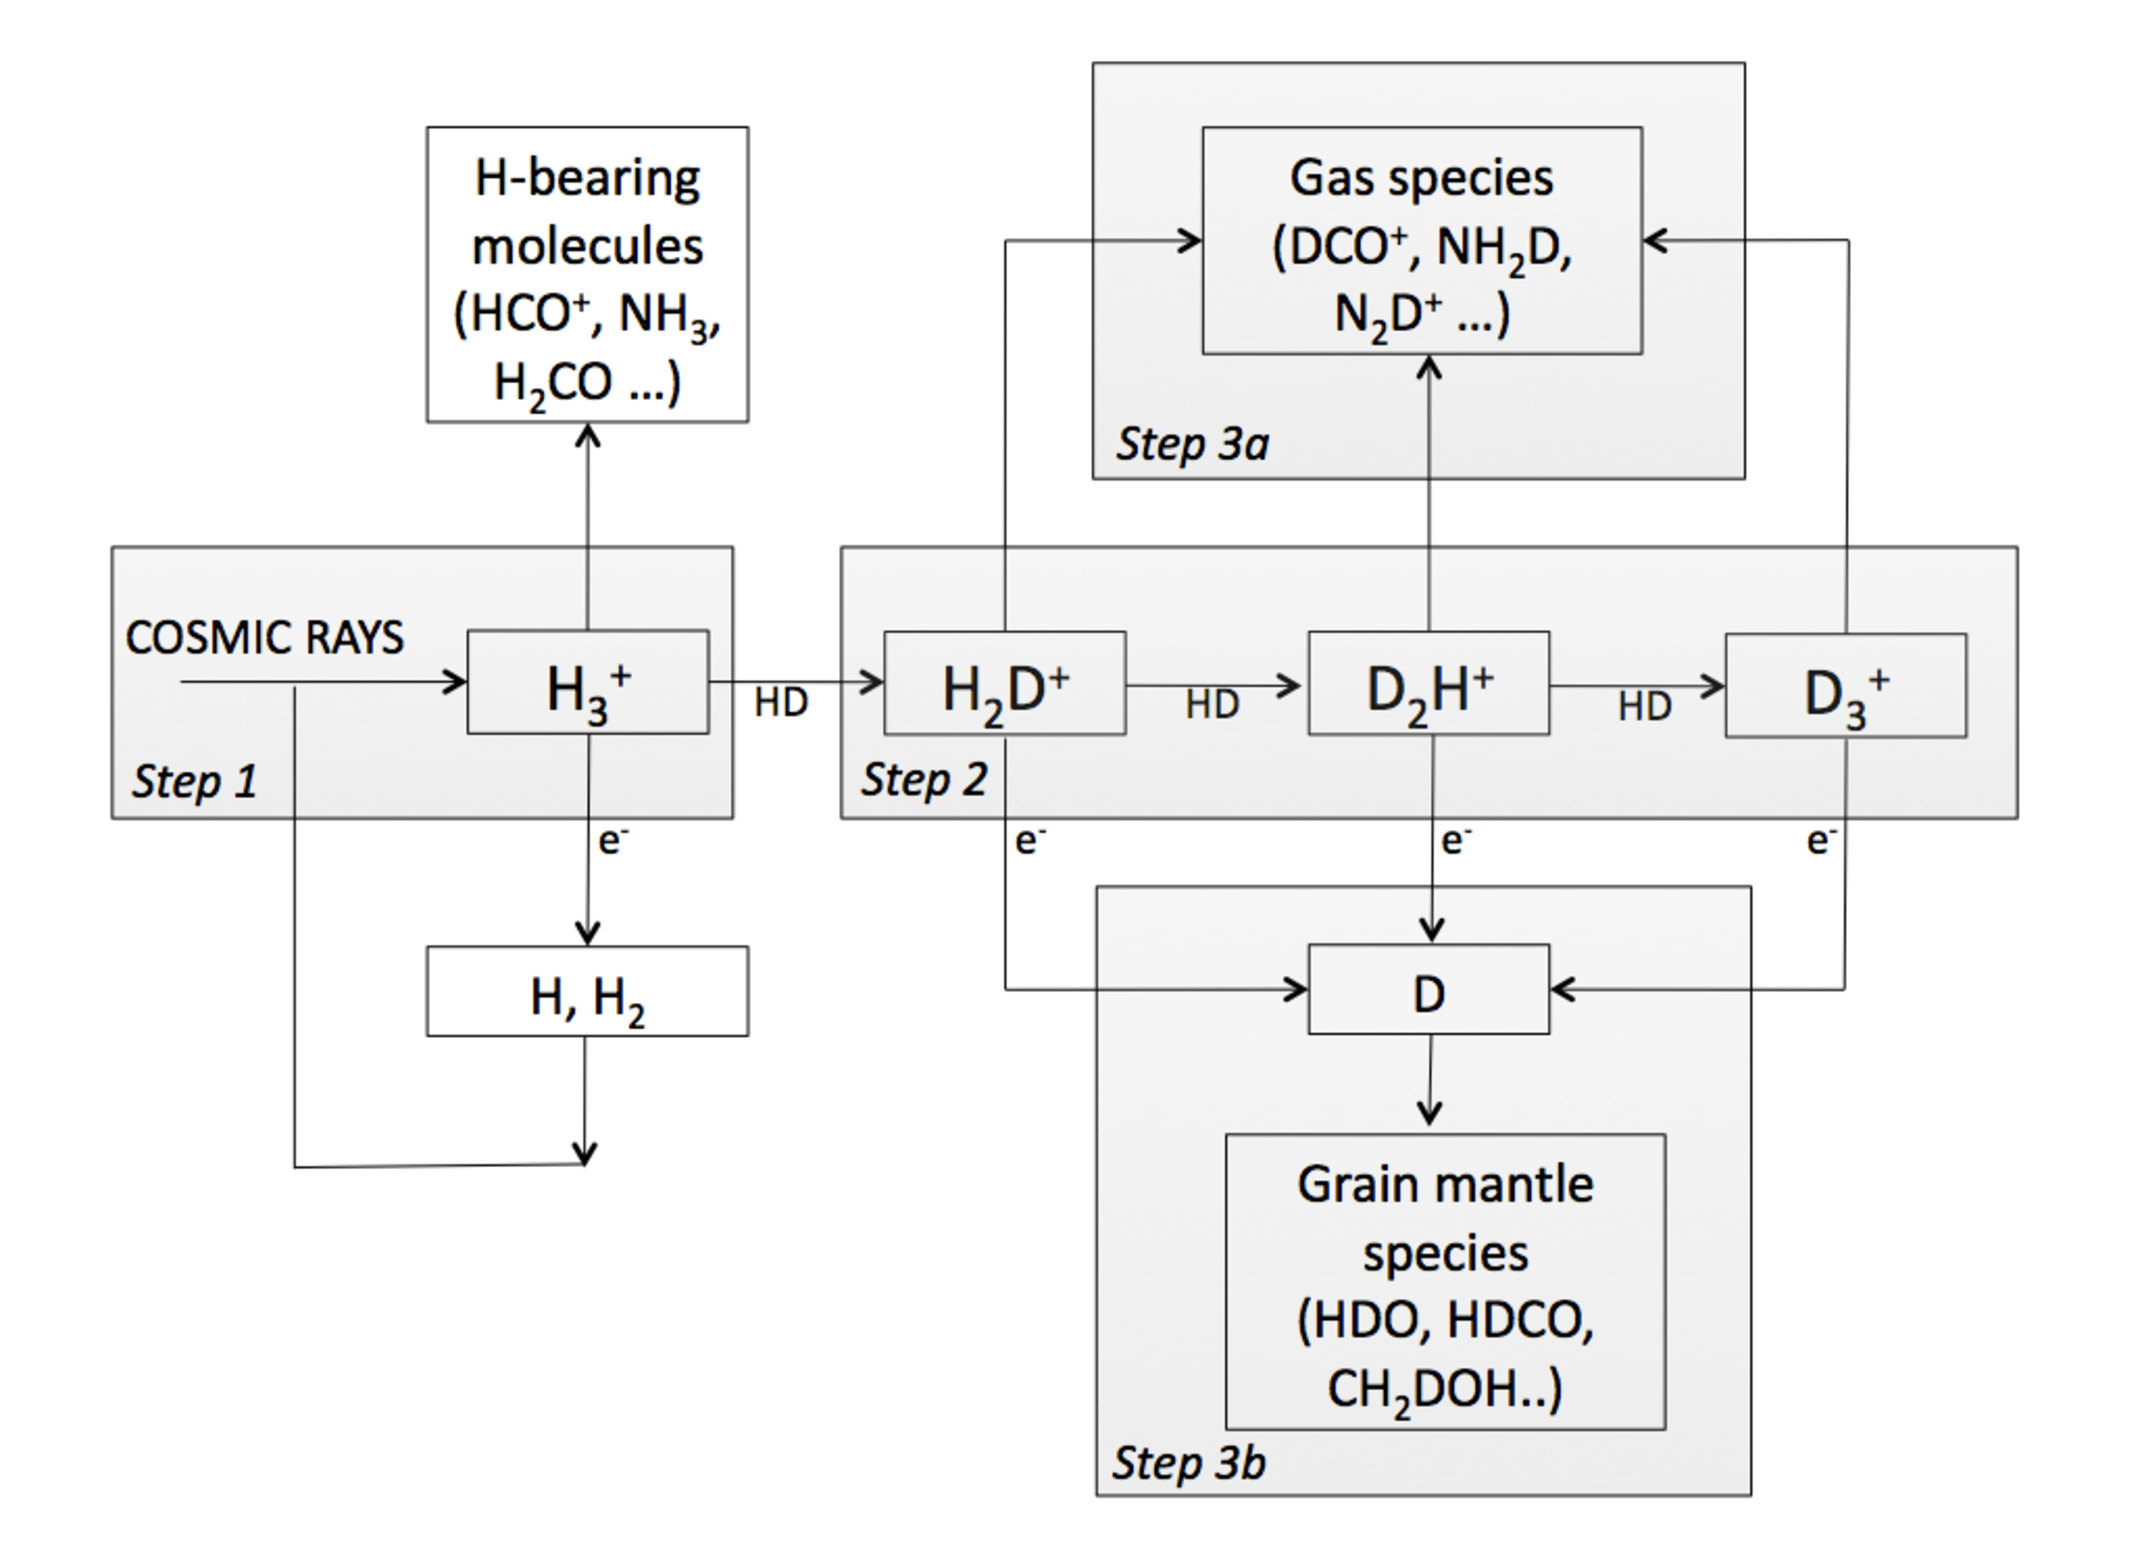
\includegraphics[width=0.9\linewidth]{kappa/images/sec2-fig1.pdf}
    \caption{Deuterium Fractionation}
    \label{fig:dfracstep}
\end{figure}

Because $\rm H_2D^+$ is the central role to transfer the D-atoms into species and its easier to exist in cold gas, deuterium fractionation is easier to be observed in cold gas. Since the formation of $\rm H_2^D+$ depends on $\rm H_3^+$, it means higher cosmis-ray ionization rate can accelerate the reactions. Besides, because $\rm H_3^+$ could be destruct by O and CO, removing these species from the gas-phase can also enhance the deuterium fractionation. That is to say, the cold and dense region like prestellar cores, where the O and CO tend to stick on grain mantles, is an ideal place for deuterium fractionation.

Another important factor influence the deuterium fractionation is the ortho-and-para ratio of molecular hydrogen ($\rm OPR^{H_2}$). The internal energy of ortho-$\rm H_2$ could overcome the barrier in the inverse reaction of Equation~\ref{eq:dfrac2ndstep} (i.e. $\rm H_2D^+ + H_2 \rightarrow H_3^+ + HD$). As a consequence, the ratio of $\rm H_2D^+/H_3^+$ is suppressed and stop the third step to occur. Theoretically, the $\rm H_2$ formed on dust grains has 75\% probability to form ortho-$\rm H_2$ and 25\% probability to for para-$\rm H_2$, but the ratio decreases in gas phase as time evolves because of proton-exchange reaction. The $\rm OPR^{H_2}$ is believed to be low in prestellar cores \cite{Sipila2013,Brunken2014}.



Observationally, $\rm N_2H^+$ and its deuterated form $\rm N_2D^+$ have been recognized as good tracers for prestellar cores. They have been oberved in L1544 and several cores in Infrared Dark Clouds.

A variety of astrochemical studies have been carried out to model deuterium fractionation. \cite{Walmsley2004} considered a reduced chemical network, including the spin states of $\rm H_2$, $\rm H_2^+$, $\rm H_3^+$ and $\rm H_2D^+$. This network assumed heavy elements, like $\rm C$, $\rm N$, $\rm O$, etc, are fully depleted. Extending this work, \cite{Flower2006}, \cite{Hugo2009}, \cite{Pagani2009} and \cite{Sipila2010} included updated reaction rates for spin states and deuterated forms of $\rm H_2$ and $\rm H_3^+$. \cite{Vastel2012} presented networks including molecular species with up to three atoms. \cite{Kong2015a} extended these works to include $\rm H_3O^+$ to acquire more precise results. As a consequence, the abundances of electrons, water, $\rm HCO^+$, $\rm DCO^+$, $\rm N_2H^+$, $\rm N_2D^+$ are improved and have a good agreement with the even more extensive network of \cite{Sipila2013}. More recently, \cite{Majumdar2016a}, based on the work of \cite{Wakelam2015}, presented a complete network including spin state chemistry with 13 elements (H, He, C, N, O, Si, So, Fe, Na, Mg, Cl, P, F).

In our work, we based on the network from \cite{Kong2015a}, which approximated the surface chemistry by gas-phase reactions.

\section{UCLCHEM}
{\UCLCHEM} \cite{Holdship2017a} is a time-dependent gas-grain chemical model written in Fortran. It extends the pure gas-phase reactions from UMIST database with gas-grain interactions including freeze-out, thermal desorption, photodesorption and cosmic-ray-induced thermal desorption based on the rate functions in \cite{Roberts2007}. To simulate the surface chemistry, it adopts an approximated way to allow users to set the branch ratio of freeze-out reactants. For example, when CO stick on grain mantles, it could be hydrogenated and form $\rm CH_3OH$. {\UCLCHEM} allows users to set, for example, 90\% CO to become grain-phase CO and the rest 10\% CO to become $\rm CH_3OH$ in their defined grain file. The whole package also includes a routine to generate the chemical modeling code and other hydrodynamics routine like C-shock and molecular clouds. However, the hydrodynamics modules are limited in single grid or one dimension.

The standard chemical network defined in {\UCLCHEM} includes hundreds of gas-grain reactions besides the 6173 gas-phase reactions. However, if we only focus on simple species like CO, $\rm H_2O$, etc, a reduced network can provide similar results as the complete network. In the simulations of ISM scale, we mainly use the reduced network generated from {\UCLCHEM}.
%binding energy?

% \lipsum[5]


% \section{Some section}

% \lipsum[3]

% \begin{figure}
% \centering
% \includegraphics[width=0.8\textwidth]{kappa/images/supervisor}
% \caption{An example of a supervisor.\label{fig:kappa-sup}}
% \end{figure}

% \lipsum[10-15]



%   .x~~"*Weu.
%  d8Nu.  9888c
%  88888  98888
%  "***"  9888%
%       ..@8*"
%    ````"8Weu
%   ..    ?8888L
% :@88N   '8888N
% *8888~  '8888F
% '*8"`   9888%
%   `~===*%"`
%
%%%%%%%%%%%%%%%%%%%%%%%%%%%%%%%
%%%%%%%%%%%%%%%%%%%%%%%%%%%%%%%
\chapter{Chemodynamics Simulation\label{ch:chemo}}
%%%%%%%%%%%%%%%%%%%%%%%%%%%%%%%

% \lipsum
% the accuracy of the main species does not change a lot (if we do not consider the updates to surface chemistry model). The advantage of more complex model is the predict more complex molecules.
Although there are more and more sophisticated astrochemical models, these models are usually implemented in one zone or one dimension. However, it means that these models ignore the kinematics influences, especially the advection diffusion induced by turbulence. To further understand the kinematics influence of the turbulence motion and even have the synthetic observations, three-dimensional chemodynamics simulations are necessary.

\section{Coupling Chemistry with Magnetohydrodynamics\label{sec:chemo}}
In a typical ideal Magnetohydrodynamics (MHD) simulation, the following equations are solved:
% \begin{equation}
%     \begin{split}
%         \frac{\partial \rho}{\partial t} + \div (\rho {\bf v}) & = 0, \\
%         \frac{\partial \rho {\bf v}}{\partial t} + \div \left(\rho {\bf v} {\bf v} + {\bf I}p^* - {\bf B} {\bf B} \right) & = - \rho {\bf v} - \rho \grad \phi, \\
%         \frac{\partial E}{\partial t} + \div \left[ (E + p^*) {\bf v} - {\bf B} ({\bf B} \cdot {\bf v}) \right] & = - \left( 2E - \frac{B^2}{2a} \right) - {\rho} {\bf v} \cdot \grad \phi  - \Lambda + \Gamma + \div {\bf F}_{\rm cond}, \\
%         \frac{\partial {\bf B}}{\partial t} - \grad \times ({\bf v} \times {\bf B}) & = 0 \\
%     \end{split}
%     % \frac{\partial \rho}{\partial t} + \nabla \cdot (\rho {\bf v}) = 0
% \end{equation}

\begin{eqnarray}
    \frac{\partial \rho}{\partial t} + \div (\rho {\bf v}) & = & 0, \label{eq:mass} \\
    \frac{\partial \rho {\bf v}}{\partial t} + \div \left(\rho {\bf v} {\bf v} + {\bf I}P - {\bf B} {\bf B} \right) & = & - \rho \grad \phi, \label{eq:momentum} \\
    \frac{\partial E}{\partial t} + \div \left[ (E + P) {\bf v} - {\bf B} ({\bf B} \cdot {\bf v}) \right] & = & - {\rho} {\bf v} \cdot \grad \phi  - \Lambda + \Gamma, \label{eq:energy} \\
    \frac{\partial {\bf B}}{\partial t} - \grad \times ({\bf v} \times {\bf B}) & = & 0 \label{eq:induction}
\end{eqnarray}

where $\rho, {\bf v}, P, E, {\bf B}, \phi$ are the density, velocity vector, pressure, energy density and magnetic field vector and potential. ${\bf I}$ is a identity tensor. $\Lambda$ and $\Gamma$ represent the radiative cooling and heating rates. To include the contribution of magnetic field, the pressure and energy are given by:
\begin{eqnarray}
    P = p + \frac{B^2}{2}, \\
    E = e + \frac{\rho v^2}{2} + \frac{B^2}{2},
\end{eqnarray}
where p and e are thermal pressure and thermal energy density. The magnetic permeability ($\mu_0$) is unity in these equations. In the case of ideal gas with a ratio of specific heats $\gamma$, the thermal energy can be given by:
\begin{equation}
    e = \frac{p}{(\gamma - 1)}
\end{equation}
If the ideal gas is isothermal, the thermal energy can also be given by sound speed ($c_s$):
\begin{eqnarray}
    c_s & = & \sqrt{\frac{\gamma kT}{\mu m_H}}  \\
    e & = & \frac{\rho c_s^2}{\gamma (\gamma-1)}
\end{eqnarray}



%complete the description of the equations


%%% copy from enzo paper
% \begin{eqnarray} 
%   \frac{\partial \rho}{\partial t} 
%   + \frac{1}{a} \div (\rho {\bf v}) & = & 0,
%   \label{eq:mass} \\
% %
%   \frac{\partial \rho {\bf v}}{\partial t}  
%   + \frac{1}{a} \div \left(\rho {\bf v} {\bf v} + {\bf I}p^* - 
%     \frac{{\bf B} {\bf B}}{a} \right) & = &
%   - \frac{\dot{a}}{a} \rho {\bf v} - \frac{1}{a} \rho \grad \phi,
%   \label{eq:momentum} \\
% %
%   \frac{\partial E}{\partial t} 
%   + \frac{1}{a} \div \left[ (E + p^*) {\bf v} - 
%     \frac{1}{a} {\bf B} ({\bf B} \cdot {\bf v}) \right] & = &
%   - \frac{\dot{a}}{a} \left( 2E - \frac{B^2}{2a} \right) - 
%   \frac{\rho}{a} {\bf v} \cdot \grad \phi 
%   - \Lambda + \Gamma + \frac{1}{a^2} \div \fcond,
%   \label{eq:total_energy}  \\
% %
%   \frac{\partial {\bf B}}{\partial t} - 
%   \frac{1}{a}  \grad \times ({\bf v} \times {\bf B}) & = & 
%   0
%   \label{eq:induction}
% \end{eqnarray}

Equations~\ref{eq:mass} $\sim$ ~\ref{eq:energy} represent the conservation of mass, momentum, and energy and Equation~\ref{eq:induction} is the magnetic induction equation. However, to extend a fluid to a reactive flow, the equation of specie evolution must to be included:
\begin{equation}
    \frac{\partial n_i}{\partial t} + \div (n_i {\bf v}) - \div ({\cal D} \grad n_i) = C(n_i, n_j, T) - D(n_j, T)n_i
    \label{eq:reactiveflow}
\end{equation}
where $n_i$ represent the number density of each species and the summation of number density weighted by mass must equal to mass density ($\displaystyle \sum_i n_i m_i = \rho$). This equation includes three processes: advection, diffusion and chemical reactions. The second and the third term in the left-hand side represent the advection and the diffusion process. In astrophysical flows, the diffusion term is usually ignored since its influence is mush smaller than advection term. The right-hand side means the construction ($C$) and destruction ($D$) of $i$th species. 


Equation~\ref{eq:reactiveflow} can be splitted into two parts:
\begin{eqnarray}
    \frac{\partial n_i}{\partial t} + \div (n_i {\bf v}) &=& 0 \\
    \frac{d n_i}{dt} &=& C(n_i, n_j, T) - D(n_j, T)n_i
\end{eqnarray}
The first equation only consider the advection term and the second equation solves the reactions, which is the same set of differential equations handled by those one-zone astrochemical model (See Chapter~\ref{ch:astrochemistry}). That is to say, to implement a chemodynamics simulation, we can make the hydrodynamics code calculate the advection and then insert the astrochemical model to solve the reactions.



% \section{\ENZO}
% % brief intro with grackle
% In our works, we mainly use ENZOv2.5 to run the simulations. ENZO was developed to run cosmological simulations. 

% \section{\KROME}
% % brief intro
% {\KROME} is a chemistry package written in Python. It works as a preprocessor to parse the chemical network provide by users and generate Fortran codes. Users have the freedom to define their own reaction format by using its pre-defined tokens.


\section{Simulation Code: \ENZO+\KROME}

In our projects, we utilize {\ENZO}\cite{Bryan2014} and {\KROME}\cite{Grassi2014a} to run the chemodynamics simulations. {\ENZO} is a adaptive mesh refinement (AMR) hydrodynamics code developed for cosmological simulations. It has built-in functions using {\tt GRACKLE} chemistry library to calculate the evolution of primordial gas. {\tt GRACKLE} also supports calculating heating/cooling rates of primordial gas and metals and some UV background radiation effects. However, the main purpose of {\tt GRACKLE} is the primordial chemistry. Although it can be extended to include some user-defined {\tt Cloudy} heating/cooling table, it is not practical to make it include a general chemical network of ISM. 

Instead, {\KROME} is a chemistry package working as a Python-based parser to convert a user-provided chemical network to Fortran codes. Users have the freedom to define their own reaction format by using its pre-defined tokens. It provides a unique interface function so that it can work with other hydrodynamics codes. However, it does not guarantee the consistency with hydrodynamics codes. Users have to ensure that all species in the network exists in the hydrodynamics codes and that the advection is handled by the hydrodynamics codes (see Section~\ref{sec:chemo}). Besides, because it generates source codes, these codes have to be compiled with the hydrodynamics codes to make it work. It also provides some official patches for several hydrodynamics codes, including {\tt FLASH, ENZO, GIZMO} and {\tt RAMSES}. For {\ENZO}, the patch does not handle the advection and the existence of species. Users have to define the additional species and modify some routines for advection and renormalization (e.g. {\tt Grid\_SolveHydroEquations.C} for PPM, Zeus, MHD\_Li/CT solvers and {\tt Grid\_UpdatePrim.C} for Runge Kutta solvers).

\section{Performance\label{sec:perform}}

Although {\KROME} provide a way to set up the codes for chemodynamics simulations, a significant problem is the size of the network. To model the chemistry happens in ISM, the networks usually contain thousands of reactions. Even if it may only take a few milliseconds to finish one step in one grid, the cost becomes significant when there are $10^6$ (the order of $128^3$ resolution) grids. Figure~\ref{fig:timescale} shows the mean time of one step of chemodynamics simulations in a $64^3$ cube. The simulations use the same initial condition but couple with different sizes of networks. Obviously, the computational time is almost proportional to the number of reactions. Note that the performance could also be influence by the initial conditions. For example, if the temperature of some grids is out of the valid range reactions, the reaction rates are zeros and could make the calculation faster. However, in general, the performance of simulations could be thousand times slower if a network containing thousands of reactions is used. 

\begin{figure}
    \centering
    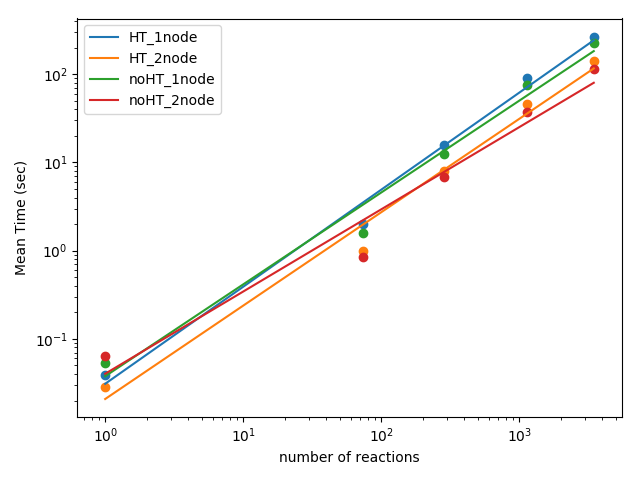
\includegraphics[width=0.8\linewidth]{kappa/images/timesize_all.png}
    \caption{Time consumption}
    \label{fig:timescale}
\end{figure}

Another problem of chemodynamics simulation is the number of species. To track the evolution and calculate the advection, the density of each species must be stored in each grid. As the number of species increases, the simulation also occupies more disk storages and memories. For example, a magnetohydrodynamics simulation usually stores about 10 fields (typically, $\rho, {\bf v}, E, {\bf B}$ and some optional fields like internal energy or potential). However, a network of ISM could contain hundreds of species. For example, if the network contains about 100 species, the simulation with the resolution of $128^3$ will use about 2GB memory. If the resolution is enhanced to $512^2$, the simulation data will exceed 100GB. The number of species limits the resolution and increase the loading of communication when the simulation running on clusters.

A simple way to save memory and disk storage is using the AMR structure to limit the finer grids focusing on subregions in the simulation. The way is effective if the interesting regions are only a small portion of the whole domain. However, the side effect is the interpolation error. Although most of popular AMR codes support high order interpolation methods and conservative interpolation to reduce the numerical error, the elementary conservation still could be broken\cite{Grassi2017}. The problem is because gradient limiters and interpolation weights could be different for each species. Even if each individual chemical species is conserved during the interpolation, the summation of atoms in species could not be conserved. This means the amount of species should be normalized twice after advection. One is for this elementary conservation and another one is for the mass conservation.

However, even if the memory requirement is affordable, the performance problem is still significant. It is unpractical to wait over fourty days for a simulation originally taking one hour. Several ways could improve the performance:
\begin{itemize}
    \item Parallelization: Parallelization is a common way to improve the performance of simulations. Currently, {\tt openmp} and {\tt MPI} have been widely applied in numerical codes. {\ENZO} also support the usage of {\tt MPI}, which can accelerate the simulation by requesting more processors from more nodes in cluster. Figure~\ref{fig:timescale} also shows the simulation is almost twice faster by using two nodes rather than one node. However, it is also unpractical to offload the heavy computation by requesting hundreds of nodes. Graphics card could be another choice of parallelization. By using the graphics processing units (GPU) on graphics cards, hydrodynamics simulations could be ten times faster than CPU\cite{Schive2010}. Note this also depends on the frequency and the number of units. Usually this kind of tests are done under the same ``cost'' of a specific cluster. Several studies are working on moving the differential equation solvers onto GPU \cite{Niemeyer2014, Curtis2016, odeint, cuda-sim(culsoda), Stone2018}. However, these studies are focusing on combustion engineering and biochemistry. They have not been ported to astrochemistry and have several drawbacks. Most solvers are explicit and cannot handle the level of stiffness in astrochemistry. Some of them use the first order BDF method and lose the accuracy. The higher order solver does not handle the sparsity matrix causes the uncertainty on performance.
    \item Reducing the size of network: Because the computational load is proportional to the number of reactions, it is intuitive to reduce the load by reducing reactions. The idea also has been studied for a long time. It can be done by pre-selecting species and related reactions\cite{Nelson1999}. Another approach assumes that some species stay on equilibrium to focus on solving the non-equilibrium species\cite{Lam1993, Glover2010}, where those equilibrium species are chosen by the rapid reaction rates. The approach may not by valid for a wide range of parameters because the float of reaction rates. A further approach then try to dynamically reduce the reactions to avoid the limitation\cite{Tupper2002, Grassi2012}.
    \item Reducing the time steps of chemistry: This could be the simplest way to accelerate the simulations, but the method only works when the chemistry timescale is much longer than the hydrodynamics timestep. If the hydrodynamics timestep is much shorter chemistry timescale, the chemistry calculation can be operated every several hydrodynamics timesteps and keep a good apprximation. This approach has been implemented in our {\ENZO} codes. However, if the simulation is under a fast heating/cooling, this approach will lose the accuracy.
    \item Neural network: Due to the advance of deep learning, neural network becomes a popular skill in a variety of fields. As the fundamental neural network, artificial neural network also has been widely applied in computational chemistry, biochemistry, etc\cite{Goncalves2013}. A recent work also apply the skill to create a emulator of {\UCLCHEM}\cite{DeMijolla2019}. As a black box, the emulator skip the cost of solving differential equation but reproduce the nonlinear results. The problems become how to train a valid model and guarantee the correctness in a wide range of parameters and whether there is a general way to train a effective model.
\end{itemize}

% neural network DeMijolla2019

%         xeee
%        d888R
%       d8888R
%      @ 8888R
%    .P  8888R
%   :F   8888R
%  x"    8888R
% d8eeeee88888eer
%        8888R
%        8888R
%     "*%%%%%%**~
%
%%%%%%%%%%%%%%%%%%%%%%%%%%%%%%%
%%%%%%%%%%%%%%%%%%%%%%%%%%%%%%%
\chapter{Introduction to Paper}
%%%%%%%%%%%%%%%%%%%%%%%%%%%%%%%

\section{Paper I}
In this paper, we focus on the deuterium fractionation in massive prestellar cores. The reason is that $\rm N_2H^+$ and its deuterated form $\rm N_2D^+$ have been oberved in several prestellar cores and are trusted to be good tracers\cite{Caselli2002, Tan2013, Kong2016}. The cold and dense gas is also an ideal place of deuterium fractionation (See Section~\ref{sec:deufrac}). Their emission lines are also useful to interpret the kinematics in the cores. As a follow-up work of \cite{Goodson2016}, we also use the chemical network in \cite{Kong2015a} but with slightly updates from \cite{Majumdar2016a}. The network contains species composed by heavy elements, C, N, and O, so that allow us to investigate the influence of depletion factor. We then use {\ENZO} and {\KROME} to couple the chemical network with magnetohydrodynamics simulation of prestellar core.

We focus on the influences of chemical parameters to an identical prestellar core. The initial conditions of the prestellar core are fixed to mass = 60 $M_{\odot}$, surface density = 0.3 $\rm gcm^{-2}$, radius = 0.1 pc. The free-fall time is expected to be 76 kyr. The prestellar core also have a velocity turbulent field and a  cylindrically symmetrical magnetic field to make the core slightly super virial in the beginning. Since there is no driving turbulence field, the core will still collapse. The chemical parameters we studied are the initial $\rm OPR^{H_2}$, temperature, cosmic-ray ionization rate and depletion factor of CO and N (two factors, one controlling the abundances of C and O, another one contral the N abundance) and their composition.

We follow the chemical evolution in the core for 0.8 free-fall time and analyze the average number densities, column densities of $\rm N_2H^+$, $\rm N_2D^+$. We conclude that one model with high cosmic-ray ionization rate ($1.0 \time 10^{-16} \rm s^{-1}$) and high depletion factor (f$_D^{CO} = 1000$, f$_D^N = 100$) is the best model matching with the observational data in our simulations. The abundances also allow us to estimate the velocity gradient, the velocity dispersion, even the rotational energy, the kinetic energy and the virial parameter of the simulated core under the assumption of optical thin of $\rm N_2D^+$(3-2) emission line. Overall, the rotational energy is little comparing with the gravitational energy, and the velocity gradient need more observational data for comparison. Besides, the core appears subvirial observationally during most time of evolution because of the contribution of magnetic field cannot be observed from velocity dispersion.



%   cuuu....uK
%   888888888
%   8*888**"
%   >  .....
%   Lz"  ^888Nu
%   F     '8888k
%   ..     88888>
%  @888L   88888
% '8888F   8888F
%  %8F"   d888"
%   ^"===*%"`
%
%%%%%%%%%%%%%%%%%%%%%%%%%%%%%%%
%%%%%%%%%%%%%%%%%%%%%%%%%%%%%%%
\chapter{Outlook}
%%%%%%%%%%%%%%%%%%%%%%%%%%%%%%%

\section{Ambipolar Diffusion in Prestellar Cores}
Following the work done in Paper~\ref{pap:psc}, we plan to include the non-ideal MHD effect, ambipolar diffusion, into the simulation. If we consider the ambipolar diffusion effect, the prestellar core could take longer time to collapse and probability a lower cosmic-ray ionization rate still can reproduce the high deuteirum fraction in observation. Also, due to the cosmic ray and depletion factors, the mean ion mass could be reduced and then enhance the ambipolar diffusion effect. 

\section{Cloud Collision}
GMC collisions are thought as a mechanism to trigger star formation. \Cite[]{Wu2015, Wu2017} has use {\ENZO} and {\tt GRACKLE} to study the influence of heating/cooling of photon dissociation region (PDR) model in GMC collisions. The heating/cooling function could help the formation of dense structures which are the progenitors of stars. The PDR model also allow the prediction of molecular lines like CO(8-7) emission line. However, these models does not really couple with chemistry and make the prediction have some uncertainty. We plan to couple the simulation with the reduced network of {\UCLCHEM} to further improve the accuracy of CO and probe other tracers of dense gas (HCN, $\rm HCO^+$). Because the gas-grain interactions are also supported by the network, it also allow us to study the depletion in dense gas. The results can be use to improve the initial condition of the prestellar core simulation.

\section{Porting astrochemical tools onto GPU}
The performance issue has been addressed in Section~\ref{sec:perform}. To run a huge network in high resolution, imporving the performance is inevitable. So far, because the chemical networks are much slower than hydrodynamics, we use the way reducing the cycle to accelerate the simulation. To further improve the performance, we would like to have a high order implicit ODE solver executable on GPU. We first plan to port the available {\tt lsoda} GPU solver to fit the requirement of astrochemistry. {\tt lsode} is another solver has been widely use and take advantage of the sparsity of matrix, but it is written in Fortran77. Porting it onto GPU could be another project. 



    \printbibliography[heading=bibintoc]

  \end{refsection}

\cleardoublepage

% % % Preparations before Part II. In this part one chapter = one paper

\renewcommand{\chaptername}{Paper}
                              % write 'Paper' instead of 'Chapter' in the title

\setcounter{chapter}{0}       % reset chapter numbers after Part I

% Fix hyperlinks to chapters/papers after chapter counter reset, see
% http://tex.stackexchange.com/a/6099
\renewcommand\theHchapter{appendedPaper.\arabic{chapter}}

\renewcommand{\thesection}{\arabic{section}}
                              % exclude chapter number from section number
                              % Figures, Tables, etc are still prefixed by chapter number.
                              % For algorithms numbering see definition of
                              % \newfloat{algorithm} above.

\newcommand{\paper}[7]
% #1 Paper Title
% #2 Short Title for page headers (ToC has the full title)
% #3 Label for later (or earlier) \ref:s
% #4 Authors
% #5 Where published
% #6 Comment (like "reprinted with a kind permission" and "reformatted for uniformity")
% #7 File to input
{
  \chapter{#1\label{#3}}      % Title as Chapter
  \chaptermark{#2}            % Short title for the page header
  \thispagestyle{empty}       % no page numbers
  {\Large #4}\par             % authors
  \vspace{1cm}
  \noindent\emph{\Large #5}\par % where published
  \vspace{3cm}
  \noindent\emph{\Large #6}   % Comment
  \cleardoublepage            % skip back side of the page
  \thispagestyle{plain}       % no header above paper title
  \begin{center}
    {\Large \bfseries Paper~\thechapter. #1}\par % title again
    \vspace{1pc}
    #4 \par                   % authors again
    \vspace{3pc}
  \end{center}
  \begin{refsection}          % start of biblatex's refsection for sub-bibliography
  \input{#7}                  % paper itself, starting from abstract (no title)
  \printbibliography[heading=subbibintoc] % biblatex bibliography
  \end{refsection}            % end of biblatex refsection
}

\newcommand{\reformatted}{The paper was reformatted for uniformity, but otherwise is unchanged.}

\part{Appended papers}        % in this part one chapter = one paper

% Example of using the command \paper defined above: 
% \paper{SAT-solving in practice, with a tutorial example from supervisory control}
%       {SAT-solving in practice, with a SCT example}
%       {pap:supervisory}
%       {Koen~Claessen, Niklas~Een, Mary~Sheeran, Niklas~Sörensson, Alexey~Voronov and Knut~Åkesson}
%       {Journal of Discrete Event Dynamic Systems (2009), 19(4): 495--524.}
%       {Reproduced with kind permission from Springer Science+Business Media. \reformatted}
%       {paper-supervisory/body}

% \paper{The same paper, inserted second time for illustration}
%       {SAT-solving in practice, with a SCT example}
%       {pap:another-one}
%       {Koen~Claessen, Niklas~Een, Mary~Sheeran, Niklas~Sörensson, Alexey~Voronov and Knut~Åkesson}
%       {Journal of Discrete Event Dynamic Systems (2009), 19(4): 495--524.}
%       {Reproduced with kind permission from Springer Science+Business Media. \reformatted}
%       {paper-supervisory/body}

\paper{Deuterium Chemodynamics of Massive Pre-stellar Cores}
      {Deuterium Chemodynamics of Massive PSCs}
      {pap:psc}
      {Chia-Jung Hsu, Jonathan C. Tan, Matthew D. Goodson, Paola Caselli, Bastian K\"{o}rtgen, Yu Cheng}
      {Accepted by MNRAS}
      { }
      {paper-supervisory/body.tex}

\end{document}
